\begin{figure*}[!t]
\centering
\begin{tikzpicture}
  \mscstart{$DE$}{$ES$};
  \mscL{holds $TID, PID, K$; fresh $N_1$ (kept in non-volatile memory); $V_1$ (E3)};
  \mscmsg{r}{$MSG_1=\{TID, N_1, V_1\}$ \ (576 bits)};
  \mscR[9.2cm]{S1 lengths; S2 find record by $I(TID)$ (E1); S3 $K$ from $C$ (E2); S4 check $V_1$ (E3)\\
        S5 fresh $N_2$; $SK$ (E4), $V_2$ (E5), $V_3$ (E6), $K'$ (E7), $TID', PID'$ (E8), $R$ (E9), $T$ (E10)\\
        \phantom{S5 }\textbf{commit}: store record over $K'$; erase old record, $K$, $R$, previous ticket;\\
        \phantom{S5 }store $T$ under the old $I(PID)$; keep pending $(SK, V_3)$};
  \mscmsg{l}{$MSG_2=\{N_2, V_2\}$ \ (416 bits)};
  \mscL[9.2cm]{D2 lengths; check $V_2$ (E5); $SK$ (E4)\\
        D3 \textbf{atomic}: $V_3$ (E6), $K'$ (E7), $TID', PID'$ (E8); store them; erase $K, TID, PID, N_1$;\\
        \phantom{D3 }DE accepts $SK$};
  \mscmsg{r}{D4: $MSG_3=\{V_3\}$ \ (256 bits)};
  \mscR{S6 $V_3$ equals the pending $V_3$: ES accepts $SK$};
  \mscend;
\end{tikzpicture}
\caption{Drone--server authentication and key establishment of FSL-AKE v3 (\texttt{spec/fsl\_ake\_v3.md}, \S6.2). S1--S6 are server steps, D2--D4 drone steps ($MSG_3$ is sent at D4); equation
numbers as in \cref{sec:scheme}. Party indices are dropped ($DE$, $ES$). No timestamps are used. Total \BitsVthree\ bits.}
\label{fig:ake}
\end{figure*}
